
\section{\label{sec:polynomialNewton}Polinom Newton}

Pada bagian ini, kita mencari proses otomatis yang efisien untuk menghitung
polinom interpolasi. Bentuk Lagrange dari polinom interpolasi paling
sesuai untuk perhitungan dengan pensil dan kertas, bukan untuk otomatisasi
komputer. Metode Neville sangat sesuai untuk menghitung nilai polinom
interpolasi pada titik tertentu, bukan untuk menghitung polinom itu
sendiri. Memang, metode Neville \textit{dapat} digunakan untuk menghitung
polinom interpolasi itu sendiri, tetapi untuk tugas ini metode tersebut
tidak lebih cocok daripada bentuk Lagrange. Dalam pembahasan berikut,
kita akan melihat bagaimana rumus rekursif yang sama dengan rumus
dalam metode Neville digunakan untuk memperoleh metode yang sangat
efisien dan cocok untuk komputer guna menghitung polinom interpolasi
itu sendiri. Hasil perhitungannya adalah sekumpulan koefisien untuk
bentuk Newton dari suatu polinom.\index{bentuk Newton}

Andaikan kita telah menghitung polinom $N_{n}(x)$ yang menginterpolasi
data 
\[
(x_{0},f(x_{0})),(x_{1},f(x_{1})),\ldots,(x_{n},f(x_{n})).
\]
Sekarang kita ingin menghitung polinom $N_{n+1}(x)$ yang menginterpolasi
data 
\[
(x_{0},f(x_{0})),(x_{1},f(x_{1})),\ldots,(x_{n+1},f(x_{n+1})),
\]
dan memanfaatkan kembali pekerjaan yang telah dilakukan (sebagaimana
kita dapat menambahkan satu titik interpolasi dalam metode Neville
dan menggunakan kembali semua pekerjaan sebelumnya)! Salah satu cara
menangani masalah ini adalah mencari polinom $q(x)$ sedemikian sehingga
\[
N_{n+1}(x)=N_{n}(x)+q(x).
\]
Agar cara ini berhasil, harus berlaku $q(x)=N_{n+1}(x)-N_{n}(x)$
untuk setiap $x$, dan khususnya $q(x_{j})=N_{n+1}(x_{j})-N_{n}(x_{j})$
untuk $j=0,1,\ldots,n+1$. Namun, $N_{n+1}(x_{j})-N_{n}(x_{j})=f(x_{j})-f(x_{j})=0$
untuk $j=0,1,\ldots,n$, sedangkan $N_{n+1}(x_{n+1})-N_{n}(x_{n+1})=f(x_{n+1})-N_{n}(x_{n+1})$.
Dengan kata lain, kita mencari polinom $q$ yang menginterpolasi titik-titik
\[
(x_{0},0),(x_{1},0),\ldots,(x_{n},0),(x_{n+1},(f-N_{n})(x_{n+1})).
\]
Ironisnya, pekerjaan ini cocok untuk bentuk Lagrange:
\begin{eqnarray}
q(x) & = & \frac{(x-x_{0})\cdots(x-x_{n})}{(x_{n+1}-x_{0})\cdots(x_{n+1}-x_{n})}(f-N_{n})(x_{n+1})\nonumber \\
 & = & \frac{(f-N_{n})(x_{n+1})}{(x_{n+1}-x_{0})\cdots(x_{n+1}-x_{n})}(x-x_{0})\cdots(x-x_{n}).\label{eq:qLagrange}
\end{eqnarray}
Namun, $\frac{(f-N_{n})(x_{n+1})}{(x_{n+1}-x_{0})\cdots(x_{n+1}-x_{n})}$
hanyalah sebuah konstanta, sehingga kita menggantinya dengan $a_{n+1}$
dan memperoleh $q(x)=a_{n+1}(x-x_{0})\cdots(x-x_{n})$. Tentu saja
kita dapat menghitung $a_{n+1}$ menggunakan rumus $\frac{(f-N_{n})(x_{n+1})}{(x_{n+1}-x_{0})\cdots(x_{n+1}-x_{n})}$,
tetapi ada cara yang lebih baik, yang segera akan kita lihat. Dari
perhitungan berikutnya kita juga dapat mengetahui bentuk yang paling
praktis untuk $N_{n}$.

Ketika $n=0$, $q$ berbentuk $a_{1}(x-x_{0})$; ketika $n=1$, $q$
berbentuk $a_{2}(x-x_{0})(x-x_{1})$; ketika $n=2$, $q$ berbentuk
$a_{3}(x-x_{0})(x-x_{1})(x-x_{2})$; dan seterusnya. Tentu saja $N_{0}(x)=a_{0}$
merupakan konstanta karena merupakan polinom interpolasi berderajat
terendah yang melalui satu titik. Jadi, $N_{1}(x)=N_{0}(x)+a_{1}(x-x_{0})$
langsung berbentuk $a_{0}+a_{1}(x-x_{0})$; $N_{2}(x)$ langsung berbentuk
$a_{0}+a_{1}(x-x_{0})+a_{2}(x-x_{0})(x-x_{1})$; $N_{3}(x)$ langsung
berbentuk $a_{0}+a_{1}(x-x_{0})+a_{2}(x-x_{0})(x-x_{1})+a_{3}(x-x_{0})(x-x_{1})(x-x_{2})$;
dan seterusnya. Hal ini menunjukkan bahwa bentuk paling praktis untuk
$N_{n+1}$, yang tidak memerlukan penyederhanaan, adalah\index{bentuk Newton}
\begin{equation}
N_{n+1}(x)=a_{0}+a_{1}(x-x_{0})+a_{2}(x-x_{0})(x-x_{1})+\cdots+a_{n+1}(x-x_{0})\cdots(x-x_{n}).\label{eq:NewtonForm}
\end{equation}
Jika dinyatakan dalam bentuk ini, besaran yang belum diketahui, $a_{n+1}$,
muncul sebagai koefisien suku $x^{n+1}$. Akibatnya, $a_{n+1}$ \textit{berpotensi}
menjadi koefisien utama $N_{n+1}$. Jika $a_{n+1}$ bernilai nol,
kita tidak menyebutnya koefisien utama. Untuk memudahkan pembahasan
selanjutnya, kita perkenalkan istilah berikut. Untuk polinom interpolasi
pada $k+1$ titik, koefisien suku $x^{k}$ disebut \textbf{koefisien
utama potensial }\index{koefisien utama potensial}(meskipun kebetulan
bernilai nol). Karena koefisien utama potensial ini merupakan inti
masalah, kita memusatkan perhatian pada penentuan koefisien utama
potensial setiap polinom interpolasi.

Di sinilah rumus rekursif
\begin{eqnarray*}
P_{i,m+1}(x) & = & \frac{(x-x_{i+m+1})P_{i,m}(x)-(x-x_{i})P_{i+1,m}(x)}{x_{i}-x_{i+m+1}}\\
P_{i,0}(x) & = & f(x_{i})
\end{eqnarray*}
yang digunakan untuk menyusun metode Neville menjadi berguna. Karena
$P_{i,m}$ dan $P_{i+1,m}$ sama-sama berderajat paling tinggi $m$,
koefisien utama potensialnya adalah koefisien suku $x^{m}$ masing-masing.
Dengan demikian, koefisien suku $x^{m+1}$ dari $(x-x_{i+m+1})P_{i,m}(x)$
sama dengan koefisien utama potensial $P_{i,m}(x)$, dan demikian
pula koefisien suku $x^{m+1}$ dari $(x-x_{i})P_{i+1,m}$ sama dengan
koefisien utama potensial $P_{i+1,m}$. Oleh karena itu, koefisien
suku $x^{m+1}$ dari $(x-x_{i+m+1})P_{i,m}(x)-(x-x_{i})P_{i+1,m}(x)$
adalah selisih antara koefisien utama potensial $P_{i,m}$ dan $P_{i+1,m}$.
Untuk menyederhanakan pembahasan, kita gunakan notasi $f_{i,j}$ untuk
koefisien utama potensial $P_{i,j}$. Dengan demikian, koefisien suku
$x^{m+1}$ dari $(x-x_{i+m+1})P_{i,m}(x)-(x-x_{i})P_{i+1,m}(x)$ hanyalah
$f_{i,m}-f_{i+1,m}$. Jadi, koefisien utama potensial $f_{i,m+1}$
dari $P_{i,m+1}$ (yakni koefisien suku $x^{m+1}$ dari $P_{i,m+1}$)
diberikan oleh
\begin{eqnarray}
f_{i,m+1} & = & \frac{f_{i,m}-f_{i+1,m}}{x_{i}-x_{i+m+1}}\label{eq:newtonRecursion}\\
f_{i,0} & = & f(x_{i}).\nonumber 
\end{eqnarray}

\noindent\begin{digression}{Beda Terbagi}

\noindent Meskipun kita memilih notasi $f_{i,j}$ untuk koefisien
utama potensial $P_{i,j}$, besaran ini jauh lebih lazim ditulis dengan
notasi lengkap $f[x_{i},x_{i+1},\ldots,x_{i+j}]$ dan disebut beda
terbagi orde $j$.\index{beda terbagi}

\noindent\end{digression}

Akhirnya, kita memperoleh rumus koefisien utama potensial yang menggunakan
kembali perhitungan sebelumnya. Karena $N_{n+1}$ dan $P_{0,n+1}$
menginterpolasi kumpulan titik yang sama dan keduanya berderajat paling
tinggi $n+1$, berdasarkan Teorema \ref{thm:interpolatingPolynomialUniqueness}
keduanya sama. Oleh karena itu, koefisien utama potensialnya, $a_{n+1}$
dan $f_{0,n+1}$, juga sama. Dari rekursi \ref{eq:newtonRecursion},
kita kemudian memperoleh $a_{n+1}=f_{0,n+1}=\frac{f_{0,n}-f_{1,n}}{x_{0}-x_{n+1}}$.

Perlu ditegaskan bahwa kita tidak menemukan polinom baru. Kita hanya
menemukan cara baru untuk menghitung polinom interpolasi yang sama.
$N_{n}$, $L_{n}$, dan $P_{0,n}$ semuanya menginterpolasi data yang
sama dan semuanya berderajat paling tinggi $n$. Oleh karena itu,
berdasarkan Teorema \ref{thm:interpolatingPolynomialUniqueness} ketiganya
sama. Hanya bentuk penulisannya yang mungkin berbeda. Bentuk polinom
dalam Persamaan \ref{eq:NewtonForm} disebut bentuk Newton.\index{bentuk Newton}

\noindent\begin{digression}{Polinom Newton}

\noindent Biasanya, bentuk Newton \index{bentuk Newton} \index{beda terbagi}
dan beda terbagi disajikan sepenuhnya terpisah dari rumus rekursif
Neville, suatu pendekatan yang memerlukan jauh lebih banyak upaya
untuk dikembangkan. Namun, ada alasan untuk melakukannya. Tidak menggunakan
rumus Neville lebih mengikuti perkembangan historis bidang ini, karena
Newton (1643--1727) mendahului Neville (1889--1961) lebih dari 200
tahun! Selain itu, mengikuti perkembangan historis secara lebih alami
mengarah pada kajian lanjutan tentang beda terbagi.

\noindent\end{digression}

\label{NewtonPolyExample}Sebagai contoh, ambil polinom yang menginterpolasi
$f(x)=e^{x}$ pada $x=0,1,2$, seperti yang kita lakukan dalam pembahasan
metode Neville \vpageref{NevillesMethodDiscussion}. $f_{0,0}=f(0)=1$,
$f_{1,0}=f(1)\approx2.718281828459045$, dan $f_{2,0}=f(2)\approx7.38905609893065$.
Jadi,
\begin{eqnarray*}
f_{0,1} & = & \frac{f_{0,0}-f_{1,0}}{x_{0}-x_{1}}=\frac{1-2.718281828459045}{0-1}\\
 &  & \approx1.718281828459045\\
f_{1,1} & = & \frac{f_{1,0}-f_{2,0}}{x_{1}-x_{2}}=\frac{2.718281828459045-7.38905609893065}{1-2}\\
 & \approx & 4.670774270471606\\
f_{0,2} & = & \frac{f_{0,1}-f_{1,1}}{x_{0}-x_{2}}=\frac{1.718281828459045-4.670774270471606}{0-2}\\
 & \approx & 1.47624622100628.
\end{eqnarray*}
Oleh karena itu, $N_{2}(x)=1+1.718281828459045(x)+1.47624622100628(x)(x-1)$.
Nilai-nilai $f_{0,i}$ merupakan koefisien $N_{n}$. Meskipun perhitungan
ini dapat dilakukan tanpa tabel, paling praktis menabulasikan nilai
$f_{i,j}$ saat nilai-nilai itu dihitung (seperti pada metode Neville).
Hal ini berlaku bagi manusia maupun komputer! Tabulasi perhitungan
memudahkan kita memahami rekursi dan membayangkan bagaimana proses
ini dapat diotomatisasi. Tabel \ref{tab:NewtonPolyExample}, yang
disebut tabel beda terbagi,\index{beda terbagi} 
\begin{table}
\hrule \caption{\label{tab:NewtonPolyExample}Contoh bentuk Newton: menghitung $N_{2}(x)$.}

\centering{}\medskip{}
\begin{tabular}{cccc}
$x_{i}$ & $f_{i,0}=f(x_{i})$ & $f_{i,1}$ & $f_{i,2}$\tabularnewline
\hline 
$0$ & $1$ & $1.718281828459045$ & $1.47624622100628$\tabularnewline
$1$ & $2.718281828459045$ & $4.670774270471606$ & \tabularnewline
$2$ & $7.38905609893065$ &  & \tabularnewline
\end{tabular}\medskip{}
\hrule 
\end{table}
 menunjukkan tabulasi tersebut. Menambahkan satu titik data pada interpolasi
semudah menghitung satu diagonal koefisien tambahan (seperti pada
metode Neville).

\subsection{Metode Sidi \index{metode Sidi}}

Sekarang kita kembali membahas metode pencarian akar Sidi berderajat
$k$, 
\[
x_{n+1}=x_{n}-\frac{g(x_{n})}{p'_{n,k}(x_{n})},
\]
dengan $p_{n,k}$ sebagai polinom interpolasi yang melalui titik-titik
\[
(x_{n},g(x_{n})),(x_{n-1},g(x_{n-1})),\ldots,(x_{n-k},g(x_{n-k})).
\]
Dalam bentuk Newtonnya,
\[
p_{n,k}(x)=g_{n,0}+g_{n-1,1}(x-x_{n})+g_{n-2,2}(x-x_{n})(x-x_{n-1})+\cdots+g_{n-k,k}(x-x_{n})\cdots(x-x_{n-k}),
\]
sehingga
\begin{equation}
p_{n,k}'(x_{n})=g_{n-1,1}+g_{n-2,2}(x_{n}-x_{n-1})+\cdots+g_{n-k,k}(x_{n}-x_{n-1})\cdots(x_{n}-x_{n-k}).\label{eq:sidisDerivative}
\end{equation}
Khususnya,
\[
p_{n,2}'(x_{n})=g_{n-1,1}+(x_{n}-x_{n-1})g_{n-2,2}
\]
dan
\[
p_{n,3}'(x_{n})=g_{n-1,1}+(x_{n}-x_{n-1})g_{n-2,2}+(x_{n}-x_{n-1})(x_{n}-x_{n-2})g_{n-3,3}
\]
, dan seterusnya. Dalam bentuk hasil kali tersarang,
\[
p_{n,k}'(x_{n})=g_{n-1,1}+(x_{n}-x_{n-1})\left[g_{n-2,2}+(x_{n}-x_{n-2})\left[\cdots+(x_{n}-x_{n-k})\left[g_{n-k,k}\right]\cdots\right]\right].
\]
Bentuk tersarang ini sangat efisien untuk diimplementasikan.

\noindent\begin{pseudocode} \index{metode Sidi!kode semu}
\begin{description}
\item [{Asumsi:}] $g$ dapat didiferensialkan $k$ kali.
\item [{Masukan:}] Nilai awal $x_{0},x_{1},\ldots,x_{k}$; entri diagonal
$g_{k,0},g_{k-1,1},\ldots,g_{0,k}$ dari tabel beda terbagi untuk
$g$.
\item [{Langkah~1:}] Tetapkan $s=g_{0,k}$;
\item [{Langkah~2:}] Untuk $i=1,2,\ldots,k-1$, kerjakan Langkah 3:

\begin{description}
\item [{Langkah~3:}] Tetapkan $s=(x_{k}-x_{i})s+g_{i,k-i}$;
\end{description}
\item [{Langkah~4:}] Tetapkan ${\displaystyle x_{k+1}=x_{k}-\frac{g_{k,0}}{s}}$;
\item [{Keluaran:}] Hampiran $x_{k+1}$.
\end{description}
\end{pseudocode} 

\noindent Kode semu ini benar sejauh yang dikerjakannya, tetapi masih
jauh dari lengkap. Kekurangan yang paling jelas ialah kode tersebut
hanya menjalankan satu langkah metode Sidi. Kekurangan yang kurang
kentara ialah jenis maupun jumlah masukannya tidak sama dengan keluarannya,
sehingga pada akhir rutin komputer masih belum siap menghitung iterasi
berikutnya. Yang kita peroleh dari rutin ini adalah $x_{k+1}$. Agar
dapat menjalankannya lagi, kita memerlukan dua larik $x_{0},x_{1},\ldots,x_{k}$
dan $g_{k,0},g_{k-1,1},\ldots,g_{0,k}$. Untuk menyiapkan larik-larik
tersebut bagi iterasi berikutnya, kita harus mengindeks ulang nilai
$x_{i}$, lalu menghitung nilai baru $g_{i,k-i}$.

\noindent\begin{pseudocode} 
\begin{description}
\item [{Asumsi:}] $g$ dapat didiferensialkan $k$ kali.
\item [{Masukan:}] Nilai awal $x_{0},x_{1},\ldots,x_{k}$; entri diagonal
$g_{k,0},g_{k-1,1},\ldots,g_{0,k}$ dari tabel beda terbagi untuk
$g$.
\item [{Langkah~1:}] Tetapkan $x_{k+1}$ menurut metode Sidi yang diterapkan
pada $x_{0},x_{1},\ldots,x_{k}$ dan $g_{k,0},g_{k-1,1},\ldots,g_{0,k}$;
\item [{Langkah~2:}] Tetapkan $g_{k+1,0}=g(x_{k+1})$;
\item [{Langkah~3:}] Untuk $i=k,k-1,\ldots,1$, lakukan Langkah 4:

\begin{description}
\item [{Langkah~4:}] Tetapkan ${\displaystyle g_{i,k+1-i}=\frac{g_{i+1,k-i}-g_{i,k-i}}{x_{k+1}-x_{i}}}$;
\end{description}
\item [{Keluaran:}] Hampiran $x_{1},\ldots,x_{k+1}$ dan entri diagonal
$g_{k+1,0},g_{k,1},\ldots,g_{1,k}$ yang bersesuaian dari tabel beda
terbagi untuk $g$.
\end{description}
\end{pseudocode} 

\noindent Kode semu baru ini, yang menggunakan kode semu sebelumnya
pada langkah pertamanya, merupakan suatu perbaikan. Kini masukan dan
keluarannya sama dalam jenis dan jumlah, sehingga keluaran rutin ini
dapat digunakan sebagai masukan bagi iterasi berikutnya. Namun, rutin
ini masih hanya menghitung satu langkah metode Sidi. Selain itu, ada
masalah lain yang selama ini kita abaikan. Setiap rutin yang sejauh
ini dituliskan dalam kode semu mengasumsikan bahwa kita telah memiliki
entri diagonal tabel beda terbagi yang bersesuaian. Tidak baik jika
pengguna kode harus memikirkan perincian ini. Rutin yang kita tulis
harus menyediakan nilai-nilai tersebut. Bagaimanapun, pengguna akhir---orang
yang berusaha mencari akar suatu fungsi---hanya akan langsung memiliki
fungsi itu dan sejumlah nilai awal. Rutin tersebut harus menyediakan
sisanya. Akhirnya, kita menyajikan kode semu dengan semangat yang
sama seperti metode-metode pencarian akar lainnya.

\noindent\begin{pseudocode} 
\begin{description}
\item [{Asumsi:}] $g$ memiliki akar di $\hat{x}$; $g$ dapat didiferensialkan
$k$ kali; $x_{0},x_{1},\ldots,x_{k}$ cukup dekat dengan $\hat{x}$.
\item [{Masukan:}] Nilai awal $x_{0},x_{1},\ldots,x_{k}$; fungsi $g$;
ketelitian yang diinginkan $tol$; jumlah maksimum iterasi $N$.
\item [{Langkah~1:}] Untuk $i=0,1,\ldots,k$, lakukan Langkah 2:

\begin{description}
\item [{Langkah~2:}] Tetapkan $g_{i,0}=g(x_{i})$;
\end{description}
\item [{Langkah~3:}] Untuk $j=1,2,\ldots,k$, lakukan Langkah 4--5:

\begin{description}
\item [{Langkah~4:}] Untuk $i=0,1,\ldots,k-j$, lakukan Langkah 5:

\begin{description}
\item [{Langkah~5:}] Tetapkan ${\displaystyle g_{i,j}=\frac{g_{i+1,j-1}-g_{i,j-1}}{x_{i+j}-x_{i}}}$
\end{description}
\end{description}
\item [{Langkah~6:}] Untuk $i=1\ldots N$, lakukan Langkah 7--11:

\begin{description}
\item [{Langkah~7:}] Hitung $x=x_{k+1}$ menurut metode Sidi yang diterapkan
pada \\
$x_{0},x_{1},\ldots,x_{k}$ dan $g_{k,0},g_{k-1,1},\ldots,g_{0,k}$;
\item [{Langkah~8:}] Jika $|x-x_{k}|\leq tol$, maka kembalikan $x$;
\item [{Langkah~9:}] Hitung $g_{k+1,0},g_{k,1},\ldots,g_{1,k}$;
\item [{Langkah~10:}] Tetapkan $x_{0}=x_{1}$; $x_{1}=x_{2}$; $\cdots$
$x_{k-1}=x_{k}$; $x_{k}=x$;
\item [{Langkah~11:}] Tetapkan $g_{k,0}=g_{k+1,0}$; $g_{k-1,1}=g_{k,1}$;
$\cdots$ $g_{0,k}=g_{1,k}$;
\end{description}
\item [{Langkah~12:}] Cetak ``Metode gagal. Jumlah maksimum iterasi terlampaui.''
\item [{Keluaran:}] Hampiran $x$ yang dekat dengan akar eksak atau pesan
kegagalan.
\end{description}
\end{pseudocode} 

\noindent Selengkap apa pun kode semu terbaru ini, masih ada satu
hal yang belum ditangani. Kode tersebut memerlukan $k$ nilai awal
untuk menjalankan metode Sidi berderajat $k$. Ketika kita menjumpai
metode sekan, kita mencatat bahwa kebutuhan akan dua nilai awal, bukan
satu, merupakan kelemahan. Kelemahan itu semakin besar dalam metode
Sidi, yang memerlukan $k+1$ nilai awal. Namun, seperti pada metode
sekan, kita dapat menghasilkan nilai awal secara otomatis jika diperlukan.
Jika metode Sidi diberi satu nilai awal, $x_{0}$, dan kita berusaha
mencari akar fungsi $g$, kita dapat menetapkan $x_{1}=x_{0}+g(x_{0})$,
seperti yang dilakukan pada metode sekan. Anda mungkin ingat bahwa
cara ini tidak terlalu berhasil. Metode sekan sering gagal konvergen
dengan pemilihan kondisi awal tersebut.

Jauh lebih sedikit yang diketahui tentang metode Sidi dan bagaimana
pemilihan nilai awal memengaruhi kekonvergenan. Menganalisis praktik
yang baik dan buruk dalam memilih nilai awal dapat menjadi proyek
yang menarik. Bagaimanapun, jika Anda memiliki nilai awal $x_{0},x_{1},\ldots,x_{j}$
dengan $1<j<k$, $k+1-j$ nilai awal yang tersisa dapat diperoleh
dengan menggunakan metode Sidi berderajat $j$ (pada $x_{0},x_{1},\ldots,x_{j}$)
untuk memperoleh $x_{j+1}$, kemudian menggunakan metode Sidi berderajat
$j+1$ (pada $x_{0},x_{1},\ldots,x_{j+1}$) untuk memperoleh $x_{j+2}$,
lalu menggunakan metode Sidi berderajat $j+2$ (pada $x_{0},x_{1},\ldots,x_{j+2}$)
untuk memperoleh $x_{j+3}$, dan seterusnya hingga $x_{k}$ dihitung.

\subsection{Octave\index{metode Sidi!kode Octave}}

Seperti halnya metode Neville, kode Octave mengikuti kode semunya
secara identik, kecuali bahwa indeks telah disesuaikan karena pengindeksan
dimulai dari 1, bukan 0.

\noindent\begin{verbatim}
%%%%%%%%%%%%%%%%%%%%%%%%%%%%%%%%%%%%%%%%%%%%%%%%%%%%
% Written by Dr. Len Brin             1 April 2014 %
% Purpose: Implementation of Sidi's Method         %
% INPUT: function g; initial values x0,x1,...,xk;  %
%        tolerance TOL; maximum number of          %
%        iterations N                              %
% OUTPUT: approximation X and number of iterations %
%        i; or message of failure                  %
%%%%%%%%%%%%%%%%%%%%%%%%%%%%%%%%%%%%%%%%%%%%%%%%%%%%
function [X,j] = sidi(x, TOL, N, g)
  n=length(x);
  for i=1:n
    G(i,1)=g(x(i));
  end%for
  for j=2:n
    for i=1:n+1-j
      G(i,j)=(G(i+1,j-1)-G(i,j-1))/(x(i+j-1)-x(i));
    end%for
  end%for
  for i=1:N
    s=G(1,n);
    for j=2:n-1
      s=(x(n)-x(j))*s+G(j,n+1-j);
    end%for
    X=x(n)-G(n,1)/s;
    if (abs(X-x(n))<TOL)
      return
    end%if
    G(n+1,1)=g(X);
    for j=n:-1:2
      G(j,n+2-j)=(G(j+1,n+1-j)-G(j,n+1-j))/(X-x(j));
    end%for
    for j=1:n-1
      x(j)=x(j+1);
    end%for
    x(n)=X;
    for j=1:n
      G(n+1-j,j)=G(n+2-j,j);
    end%for
  end%for
  X = "Method failed. Maximum iterations exceeded.";
end%function
\end{verbatim}\texttt{sidi.m} dapat diunduh dari \href{http://lqbrin.github.io/tea-time-numerical/ancillaries.html}{situs pendamping}.

\subsection{Beda terbagi lebih lanjut\index{beda terbagi}}

Tabel beda terbagi umumnya dihitung untuk mencari koefisien satu polinom
interpolasi, dan hanya satu polinom interpolasi. Namun, setiap tabel
beda terbagi sarat dengan representasi berbagai polinom interpolasi.
Salah satu keunggulan tabel beda terbagi ialah entrinya dapat digunakan
kembali apabila data baru ditambahkan. Sifat yang sama dapat dipandang
secara terbalik. Misalkan Anda memiliki tabel beda terbagi yang dihitung
dari 4 nilai data, tetapi hanya tertarik pada polinom interpolasi
berderajat paling tinggi 2. Tabel beda terbagi tersebut

\begin{center}
\begin{tabular}{c|cccc}
$x_{0}$ & $f_{0,0}$ & $f_{0,1}$ & $f_{0,2}$ & $f_{0,3}$\tabularnewline
$x_{1}$ & $f_{1,0}$ & $f_{1,1}$ & $f_{1,2}$ & \tabularnewline
$x_{2}$ & $f_{2,0}$ & $f_{2,1}$ &  & \tabularnewline
$x_{3}$ & $f_{3,0}$ &  &  & \tabularnewline
\end{tabular}
\par\end{center}

\noindent sebenarnya memberi kita dua polinom interpolasi berbeda
berderajat paling tinggi dua, masing-masing dengan empat representasi!
Pertama, tabel tersebut dirancang untuk menghitung polinom interpolasi
\[
P_{3}(x)=f_{0,0}+f_{0,1}(x-x_{0})+f_{0,2}(x-x_{0})(x-x_{1})+f_{0,3}(x-x_{0})(x-x_{1})(x-x_{2}).
\]
Perhatikan bahwa jika kita hanya menghapus suku $f_{0,3}(x-x_{0})(x-x_{1})(x-x_{2})$
tersebut, kita masih memiliki polinom interpolasi dengan simpul $x_{0},x_{1},x_{2}$.
Klaim ini dapat didukung setidaknya dengan dua cara. Pertama, suku
$f_{0,3}(x-x_{0})(x-x_{1})(x-x_{2})$ bernilai $0$ pada $x_{0},x_{1},x_{2}$
sehingga tidak berkontribusi pada interpolasi di simpul $x_{0},x_{1},x_{2}$.
Kedua, kita dapat ``merekayasa balik'' tabel itu dengan hanya menghapus
diagonal paling bawah. Tabel yang tersisa tetap merupakan tabel beda
terbagi yang sah karena tidak ada entri yang tersisa bergantung pada
entri yang dihapus:

\begin{center}
\begin{tabular}{c|ccc}
$x_{0}$ & $f_{0,0}$ & $f_{0,1}$ & $f_{0,2}$\tabularnewline
$x_{1}$ & $f_{1,0}$ & $f_{1,1}$ & \tabularnewline
$x_{2}$ & $f_{2,0}$ &  & \tabularnewline
\end{tabular}
\par\end{center}

\noindent Jadi 
\[
P_{2}(x)=f_{0,0}+f_{0,1}(x-x_{0})+f_{0,2}(x-x_{0})(x-x_{1})
\]
merupakan salah satu polinom interpolasi berderajat paling tinggi
2. Menghapus baris teratas tabel juga menyisakan tabel beda terbagi
yang sah:

\begin{center}
\begin{tabular}{c|ccc}
$x_{1}$ & $f_{1,0}$ & $f_{1,1}$ & $f_{1,2}$\tabularnewline
$x_{2}$ & $f_{2,0}$ & $f_{2,1}$ & \tabularnewline
$x_{3}$ & $f_{3,0}$ &  & \tabularnewline
\end{tabular}
\par\end{center}

\noindent sehingga
\[
Q_{2}(x)=f_{1,0}+f_{1,1}(x-x_{1})+f_{1,2}(x-x_{1})(x-x_{2})
\]
merupakan polinom interpolasi lain berderajat paling tinggi 2. Perhatikan
bahwa $P_{2}$ dan $Q_{2}$ bukan sekadar representasi berbeda dari
polinom yang sama. Keduanya adalah dua polinom yang berbeda! $P_{2}$
menginterpolasi pada simpul $x_{0},x_{1},x_{2}$ sedangkan $Q_{2}$
menginterpolasi pada simpul $x_{1},x_{2},x_{3}$. 

Diagonal paling bawah dari setiap tabel yang dipangkas juga memberikan
polinom interpolasi berderajat paling tinggi 2. Ingat bahwa $f_{i,j}$
menyatakan koefisien utama potensial polinom interpolasi pada simpul
$x_{i},x_{i+1},\ldots,x_{i+j}$. Oleh karena itu, 
\[
\tilde{Q}_{2}(x)=f_{3,0}+f_{2,1}(x-x_{3})+f_{1,2}(x-x_{3})(x-x_{2})
\]
menginterpolasi pada simpul $x_{3},x_{2},x_{1}$ dan
\[
\tilde{P}_{2}(x)=f_{2,0}+f_{1,1}(x-x_{2})+f_{0,2}(x-x_{2})(x-x_{1})
\]
menginterpolasi pada simpul $x_{2},x_{1},x_{0}$. Keduanya bukan polinom
baru. Keduanya merupakan representasi baru untuk $P_{2}$ dan $Q_{2}$.
Tepatnya, $\tilde{P}_{2}=P_{2}$ dan $\tilde{Q}_{2}=Q_{2}$. 

Ciri penting setiap representasi polinom interpolasi ini ialah bahwa
setiap koefisien berturut-turut bergantung pada semua simpul yang
sama dengan koefisien sebelumnya, ditambah satu simpul baru. Sebagai
contoh, $f_{2,0}$ bergantung pada $x_{2}$, $f_{1,1}$ bergantung
pada $x_{2}$ dan $x_{1}$, sedangkan $f_{0,2}$ bergantung pada $x_{2}$,
$x_{1}$, dan $x_{0}$. Oleh karena itu, ketiga koefisien ini dapat
digunakan untuk menghasilkan polinom interpolasi pada simpul $x_{0},x_{1},x_{2}$
dalam bentuk polinom $\tilde{P}_{2}$ (yang, seperti telah kita catat,
sama dengan $P_{2}$). Representasi lain untuk polinom yang sama dapat
ditulis dengan menggunakan $f_{1,0}$ (yang bergantung pada $x_{1}$),
$f_{0,1}$ (yang bergantung pada $x_{1}$ dan $x_{0}$), serta $f_{0,2}$
(yang bergantung pada $x_{1},x_{0},x_{2}$):
\[
\hat{P}_{2}(x)=f_{1,0}+f_{0,1}(x-x_{1})+f_{0,2}(x-x_{1})(x-x_{0})
\]
sehingga memberikan representasi polinom yang menginterpolasi pada
$x_{0},x_{1},x_{2}$ (yang dengan demikian harus sama dengan $P_{2}$).
Ada satu representasi lain dari $P_{2}$ yang dapat diambil dari tabel
beda terbagi semula. Representasi itu berasal dari koefisien $f_{1,0},f_{1,1},f_{0,2}$.
Dapatkah Anda menuliskannya? Jawaban \vpageref{que:p2}. Ada dua representasi
lain dari $Q_{2}$ yang dapat diambil dari tabel beda terbagi semula.
Dapatkah Anda menuliskannya? Jawaban \vpageref{que:q2}.

\noindent\begin{small}

\subsection{Konsep Utama}
\begin{description}
\item [{Bentuk~Newton~untuk~suatu~polinom~interpolasi:}] \index{bentuk Newton}Bentuk
Newton, $N_{n}$, dari polinom berderajat paling tinggi $n$ yang
menginterpolasi titik-titik $(x_{0},y_{0}),(x_{1},y_{1}),\ldots,(x_{n},y_{n})$
adalah 
\[
N_{n}(x)=a_{0}+a_{1}(x-x_{i_{0}})+a_{2}(x-x_{i_{0}})(x-x_{i_{1}})+\cdots+a_{n}(x-x_{i_{0}})\cdots(x-x_{i_{n-1}})
\]
untuk $n$ indeks berbeda $i_{0},i_{1},\ldots,i_{n-1}$ dari himpunan
$\{0,1,2,\ldots,n\}$. Bentuk Newton untuk suatu kumpulan data tertentu
tidak bersifat unik.
\item [{Koefisien~utama~potensial:}] \index{koefisien utama potensial}Untuk
polinom interpolasi pada $k+1$ titik, koefisien suku $x^{k}$ disebut
koefisien utama potensialnya.
\item [{Beda~terbagi:}] \index{beda terbagi}Koefisien bentuk Newton dari
suatu polinom interpolasi disebut beda terbagi.
\end{description}

\subsection{Latihan}
\begin{enumerate}
\item Ubahlah kode semu metode Neville \vpageref{NevillesMethodPseudoCode}
agar menghasilkan kode semu untuk menghitung koefisien $N_{n}$.
\item \label{exc:interpolation-newton-3}\octave\ Ubahlah kode Octave metode
Neville \vpageref{NevillesMethodOctaveCode} agar menghasilkan kode
Octave untuk menghitung koefisien $N_{n}$. Ujilah kode tersebut dengan
menghitung $N_{2}$ yang menginterpolasi $f(x)=e^{x}$ pada $x=0,1,2$
dan membandingkan hasil Anda dengan hasil pada \vpageref{NewtonPolyExample}.
\item Misalkan $f(0.1)=0.12,\ f(0.2)=0.14,\ f(0.3)=0.13$, dan $f(0.4)=0.15$.

\begin{enumerate}
\item Carilah koefisien utama polinom berderajat terendah yang menginterpolasi
data tersebut.
\item Misalkan juga bahwa $f(0.5)=0.11$. Gunakan hasil sebelumnya untuk
mencari koefisien utama polinom berderajat terendah yang menginterpolasi
seluruh data.
\end{enumerate}
\item \label{exc:interpolation-newton-4}Carilah bentuk Newton dari polinom
berderajat paling tinggi 3 yang menginterpolasi titik-titik $(1,2)$,
$(2,2)$, $(3,0)$ dan $(4,0)$. \hasasolution 
\item \label{exc:interpolation-newton-5}Gunakan metode beda terbagi untuk
mencari polinom berderajat paling tinggi dua yang menginterpolasi
titik-titik $(0,10)$, $(30,58)$, $(1029,-32)$. \hasananswer 
\item \label{exc:interpolation-newton}Gunakan beda terbagi untuk mencari
polinom interpolasi bagi data $f(1)=0.987$, $f(2.2)=-0.123$, dan
$f(3)=0.432$. \hasasolution 
\item Buatlah tabel beda terbagi untuk data berikut hanya dengan menggunakan
pensil dan kertas.
\[
f(1.2)=2.2\quad f(1.4)=2.1\quad f(1.6)=2.3
\]

\begin{enumerate}
\item Apa polinom interpolasi berderajat paling tinggi 2 tersebut? Apakah
derajatnya benar-benar 2?
\item Tuliskan dua polinom interpolasi linear yang berbeda untuk data ini
berdasarkan tabel Anda.
\end{enumerate}
\item \label{exc:interpolation-newton-6}Gunakan beda terbagi untuk mencari
polinom berderajat paling tinggi tiga dari latihan \ref{exc:interpolation-lagrange-1}
pada bagian \ref{sec:polynomialLagrange}. Apakah derajatnya sesuai
dengan yang diharapkan? \hasananswer 
\item \label{exc:interpolation-newton-2}Carilah polinom interpolasi berderajat
paling tinggi dua yang berbentuk 
\[
p_{n}(x)=a_{0}+a_{1}(x-x_{0})+a_{2}(x-x_{0})(x-x_{1})+\cdots+a_{n}(x-x_{0})(x-x_{1})\cdots(x-x_{n-1})
\]
untuk data dalam tabel.

\begin{center}
\begin{tabular}{c|ccc}
$i$ & $0$ & $1$ & $2$\tabularnewline
\hline 
$x_{i}$ & $2$ & $3$ & $4$\tabularnewline
$f(x_{i})$ & $3$ & $5$ & $4$\tabularnewline
\end{tabular}
\par\end{center}
\item \label{exc:interpolation-newton-7}\octave\ Gunakan kode Octave dari
soal \ref{exc:interpolation-newton-3} untuk menghitung polinom interpolasi
berderajat paling tinggi empat bagi data berikut:

\begin{center}
\begin{tabular}{c|c}
$x$ & $f(x)$\tabularnewline
\hline 
$0.0$ & $-6.00000$\tabularnewline
$0.1$ & $-5.89483$\tabularnewline
$0.3$ & $-5.65014$\tabularnewline
$0.6$ & $-5.17788$\tabularnewline
$1.0$ & $-4.28172$\tabularnewline
\end{tabular}
\par\end{center}

Kemudian tambahkan $f(1.1)=-3.9958$ ke tabel dan hitung polinom interpolasi
berderajat paling tinggi 5 dengan menggunakan kalkulator. Anda dapat
menggunakan kode Octave untuk memeriksa pekerjaan Anda. \hasasolution 
\item \label{exc:interpolation-newton-1}\octave\ Gunakan kode Octave dari
soal \ref{exc:interpolation-newton-3} untuk mencari polinom interpolasi
berderajat paling tinggi satu, dua, dan tiga bagi data berikut. Hampiri
$f(8.4)$ dengan menggunakan setiap polinom.
\[
\begin{gathered}f(8.1)=16.94410,\ f(8.3)=17.56492,\\
f(8.6)=18.50515,\ f(8.7)=18.82091
\end{gathered}
\]
\item \label{exc:interpolation-newton-8}Carilah batas galat penggunaan
polinom interpolasi dari soal \ref{exc:interpolation-newton} untuk
menghampiri $f(2)$ dengan mengasumsikan bahwa semua turunan $f$
dibatasi di antara $-2$ dan $1$ pada interval $[1,3]$. \hasasolution 
\item Mengenai polinom pada soal \ref{exc:interpolation-newton-2},

\begin{enumerate}
\item gunakan polinom tersebut untuk menghampiri $f(2.5)$; dan
\item dengan mengasumsikan $f\in C^{3}$, carilah batas teoretis galat dalam
menghampiri $f(x)$ pada interval $[2,4]$.
\end{enumerate}
\item \label{exc:interpolation-newton-9} \hasananswer 

\begin{enumerate}
\item Carilah batas galat dalam bentuk $f^{(4)}(\xi_{8.4})$ bagi hampiran
$P_{3}(8.4)$ pada soal \ref{exc:interpolation-newton-1}.
\item Carilah batas galat dalam bentuk $f^{(4)}(x)$ bagi hampiran $P_{3}(x)$
pada soal \ref{exc:interpolation-newton-1} yang berlaku untuk setiap
$x\in[8.1,8.7]$.
\item Misalkan $f^{(4)}(x)=x\cos x-e^{x}$ untuk fungsi $f(x)$ pada soal
\ref{exc:interpolation-newton-1}. Gunakan informasi ini untuk mencari
batas galat bagi hampiran $P_{3}(x)$ yang berlaku untuk setiap $x\in[8.1,8.7]$.
\end{enumerate}
\item \label{exc:interpolation-newton-10}Buck menumpahkan kopi pada tabel
beda terbaginya sehingga beberapa angka menjadi tak terbaca. Meskipun
demikian, masih ada cukup informasi yang terbaca untuk mencari polinom
berderajat paling tinggi 3 yang menginterpolasi data tersebut. Carilah
polinom itu. \hasananswer 

\begin{center}
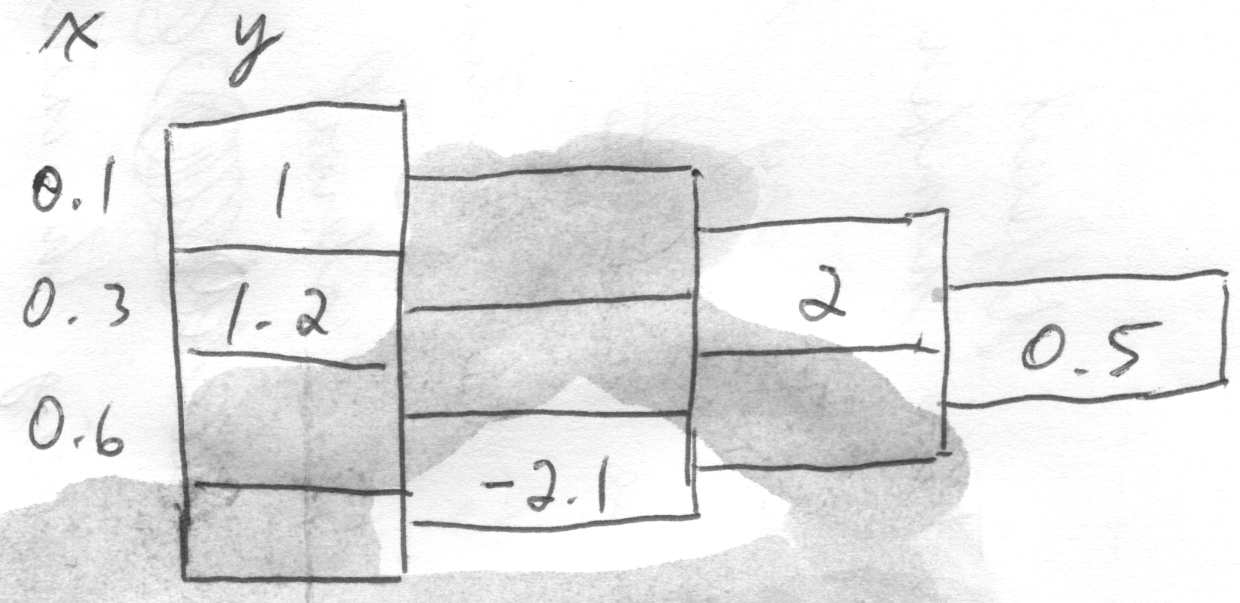
\includegraphics[width=6cm]{figures/interpolation-newton1}
\par\end{center}
\item Tunjukkan bahwa polinom yang menginterpolasi data berikut berderajat
3.

\begin{center}
\begin{tabular}{c|cccccc}
$x$ & $-2$ & $-1$ & $0$ & $1$ & $2$ & $3$\tabularnewline
\hline 
$f(x)$ & $1$ & $4$ & $11$ & $16$ & $13$ & $-4$\tabularnewline
\end{tabular}
\par\end{center}
\item \label{exc:interpolation-newton-11}Untuk fungsi $f$, rumus beda
terbagi Newton memberikan polinom interpolasi
\[
N_{3}(x)=1+4x+4x(x-0.25)+\frac{16}{3}x(x-0.25)(x-0.5)
\]
pada simpul $x_{0}=0$, $x_{1}=0.25$, $x_{2}=0.5$, $x_{3}=0.75$.
Carilah $f(0.75)$. \hasasolution 
\item \label{exc:interpolation-newton-12}Pasangkan fungsi dengan diagram
kekonvergenan metode Sidi dengan satu nilai awal. Dalam setiap kasus,
metode Sidi berderajat $6$ digunakan. Sumbu riil melewati pusat setiap
diagram, sedangkan sumbu imajiner ditampilkan, tetapi tidak selalu
berada di tengah. \hasasolution  
\begin{eqnarray*}
f(x) & = & \sin x\\
g(x) & = & \sin x-e^{-x}\\
h(x) & = & e^{x}+2^{-x}+2\cos x-6\\
l(x) & = & 56-152x+140x^{2}-17x^{3}-48x^{4}+9x^{5}
\end{eqnarray*}

\begin{center}
\begin{tabular}{cccc}
(a) &  & (b) & \tabularnewline
 & 
\includegraphics[scale=0.4]{figures/interpolation-newton2} &  & 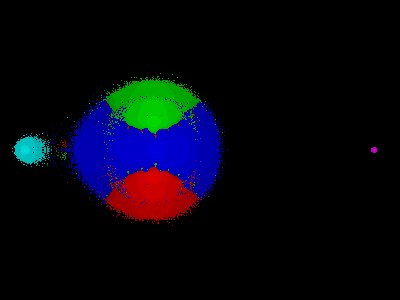
\includegraphics[scale=0.4]{figures/interpolation-newton5}\tabularnewline
(c) &  & (d) & \tabularnewline
 & 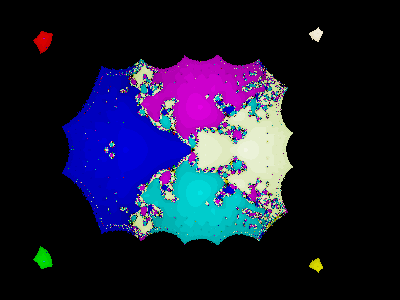
\includegraphics[scale=0.4]{figures/interpolation-newton4} &  & 
\includegraphics[scale=0.4]{figures/interpolation-newton3}\tabularnewline
\end{tabular}
\par\end{center}
\item \label{exc:interpolation-newton-13}Pasangkan fungsi dengan diagram
kekonvergenan metode Sidi dengan satu nilai awal. Sumbu riil melewati
pusat setiap diagram, sedangkan sumbu imajiner ditampilkan, tetapi
tidak selalu berada di tengah. \hasananswer 
\begin{eqnarray*}
f(x) & = & x^{4}+2x^{2}+4\\
g(x) & = & (x^{2})(\ln x)+(x-3)e^{x}\\
h(x) & = & 1+2x+3x^{2}+4x^{3}+5x^{4}+6x^{5}\\
l(x) & = & (\ln x)(x^{3}+1)
\end{eqnarray*}

\begin{center}
\begin{tabular}{cccc}
(a) &  & (b) & \tabularnewline
 & 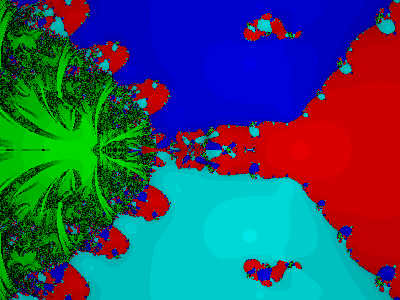
\includegraphics[scale=0.4]{figures/interpolation-newton8} &  & 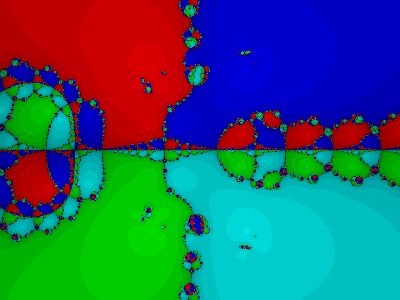
\includegraphics[scale=0.4]{figures/interpolation-newton9}\tabularnewline
(c) &  & (d) & \tabularnewline
 & 
\includegraphics[scale=0.4]{figures/interpolation-newton6} &  & 
\includegraphics[scale=0.4]{figures/interpolation-newton7}\tabularnewline
\end{tabular}
\par\end{center}
\item Anda menemukan fungsi Octave berikut tanpa komentar (penulis fungsi
itu patut dicela!).

\begin{verbatim}
function ans = foo(x,y,x0)
  n = length(x);
  ans = 0;
  for i=1:n
    a=1;
    for j=1:n
      if (j==i)
        a=a*y(i);
      else
        a=a*(x0-x(j))/(x(i)-x(j));
      endif
    endfor
    ans=ans+a;
  endfor
endfunction
\end{verbatim}

Apa keluaran (\texttt{ans}) dari perintah Octave

\begin{center}
\texttt{foo({[}1.1,1.2,1.3,1.4{]},{[}.78,.81,.79,.75{]},1.2)} 
\par\end{center}

dan mengapa?
\end{enumerate}
\noindent\end{small}

\subsection{Jawaban}
\begin{description}
\item [{$P_{2}$~dari~$f_{1,0},f_{1,1},f_{0,2}$:}] \label{que:p2}$\overline{P}_{2}(x)=f_{1,0}+f_{1,1}(x-x_{1})+f_{0,2}(x-x_{1})(x-x_{2})$
\item [{$Q_{2}$~dua~cara~baru:}] \label{que:q2}$\hat{Q}_{2}(x)=f_{2,0}+f_{1,1}(x-x_{2})+f_{1,2}(x-x_{2})(x-x_{1})$
dan $\overline{Q}_{2}(x)=f_{2,0}+f_{2,1}(x-x_{2})+f_{1,2}(x-x_{2})(x-x_{3})$
\end{description}

